\documentclass[tikz,border=10pt]{standalone}
\usepackage{amsmath}
\begin{document}
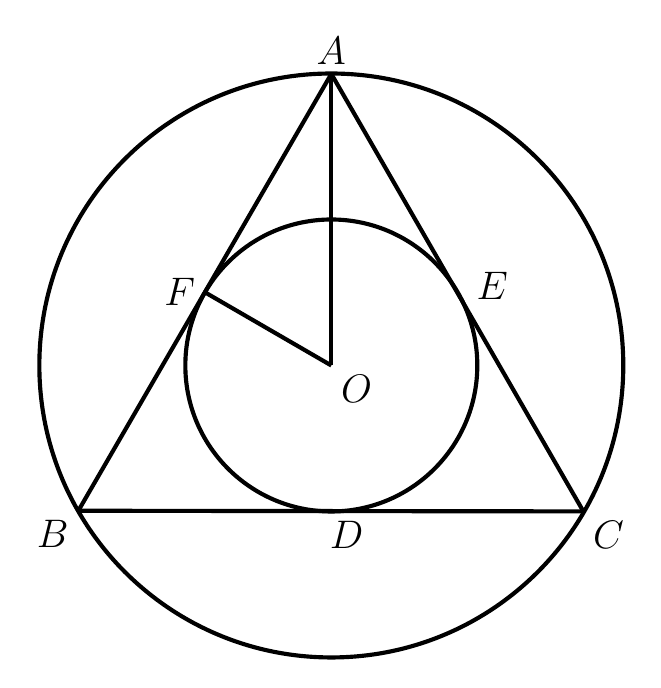
\begin{tikzpicture}[line join=round]
\coordinate (A) at (0.000,3.371);
\coordinate (B) at (-3.213,-2.177);
\coordinate (C) at (3.201,-2.185);
\coordinate (D) at (0.194,-2.184);
\coordinate (F) at (-1.606,0.598);
\coordinate (O) at (0.000,-0.332);









\coordinate (E) at (1.721,0.382);


\draw[line width=1.5pt] (O) circle (3.708);
\draw[line width=1.5pt] (O) circle (1.854);


\draw[line width=1.5pt] (A) -- (B);
\draw[line width=1.5pt] (A) -- (C);
\draw[line width=1.5pt] (B) -- (C);


\draw[line width=1.5pt] (A) -- (O);
\draw[line width=1.5pt] (O) -- (F);


\node[above] at (A) {\fontsize{15.5}{18.6}\selectfont $A$};
\node[below left] at (B) {\fontsize{15.5}{18.6}\selectfont $B$};
\node[below right] at (C) {\fontsize{15.5}{18.6}\selectfont $C$};
\node[below right] at (O) {\fontsize{15.5}{18.6}\selectfont $O$};
\node[left] at (F) {\fontsize{15.5}{18.6}\selectfont $F$};
\node[above right] at (E) {\fontsize{15.5}{18.6}\selectfont $E$};
\node[below] at (D) {\fontsize{15.5}{18.6}\selectfont $D$};
\end{tikzpicture}
\end{document}